\chapter{Game Design}
\section{Reminder}
\section{New Data}
As new services and new technologies enter the market of social medias, people keep changing the way they make use of said products. A lot of the platforms focus on giving more incentive to their users to expose a larger and larger part of their life on said services as it is at the core of their business to increase the usage of their product. They develop new ways for people to share their experiences and it gives social medias the ability to be a part of the everyday life of a lot of their users. Facebook is no exception to this, the more the people can share, the more they will use the platform and interact with their friends on it and the more likely they are to come back. To be able to exploit those resources as much as possible in ReminisceMe we must continuously be on the look for new ways we can update and refine our data model to improve our understanding of biographical memory.
\subsection{New reactions}
Since the 24\textsuperscript{th} of February 2016 \cite{reactrelease}, Facebook has introduced five new possible reactions to a post they see on their feed. These reactions complement the "Like" reaction which has been for years the only possible reaction. The five new reactions are "Love", "Haha", "Wow", "Sad" and "Angry". The primary goal here is to make sure the user can express more emotions easily (before that you had to write something as a comment to express anything else than  a like). Therefore, it will potentially improve the quality of the data we get as the user is more likely to provide more nuance now. It is important for this project to take those into account said nuances have will have a definite impact on how the user remembers the posts and interaction on the platform. These new reactions are therefore now collected by the latest version of ReminisceMe.\\
To exploit this new source of information, we decided to add two sort of questions to the existing ones.
\paragraph{Who loved/laughed at/was impressed by/was sad about/was angry at this post you made?}
Following the same schema as "Who liked this post you made?", those are the most obvious choices. What we get from those is a bit of nuance, it helps showing if the player not only remembers someone they interacted with but the way the interaction happened. In order to make them  recognizable in one quick glance, we display the image corresponding to the type of reaction next to the question text. 
\paragraph{Order the reactions on this post according to their number}
This question can be really trivial to answer in a lot of cases because in most cases a post generates mainly on type of reaction and the other are negligible. This happens because we tend to befriend people who mostly share the same opinions as we do and when we share something because we find it lovely, amusing, awesome, sad or revolting, the majority of people seeing it will share the same reaction as ourselves. However, in some instances, a post will generate a lot of polemic and the people will have a lot of intense discussion about it ((especially if we are talking about politics or religion), resulting in a multitude of different reactions. In that instance, asking to order the reactions tells us if the user remembers about the discussion around that post, if the once seemingly hot topic is still in their mind and if they remember how their friend reacted to it.\\
A caveat would be that in some cases the question is made artificially hard because some of the reactions are two similar. For instance, if the post is about a funny video, you might get nearly as much "LIKE" as "HAHA" because a lot of people laughed at the video but half of them used the "LIKE" button to express their appreciation. In that case, even knowing that the post made a positive impression, it might be really hard to answer.\\
An other issue is that the amount of people using a reaction that is not a "LIKE" might be still rather small. The feature being quite recent, a lot of the people we tested are still not used to the new reactions being there and use them a lot less than the "LIKE" which has been at the core of the Facebook experience for so long. In order to properly measure the impact of those new reactions we would need to find users who are actively using a lot of them. This being said, we felt that it was really important to start experimenting anyway because it adds to the diversity of questions and it helps generating more interesting game boards.\\
Figure \ref{fig:reactOrder} shows an example of this new kind of question.
\begin{figure}[!h]
\center
{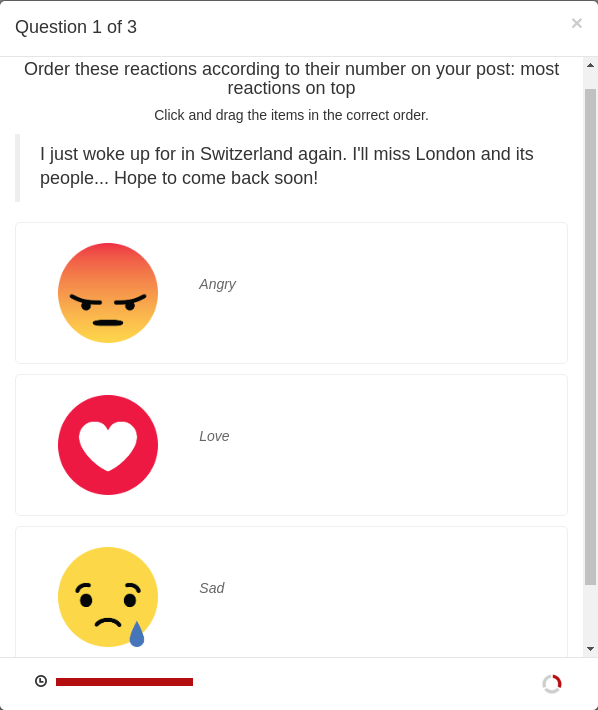
\includegraphics[width=3.5in]{images/order_reactions.png}}
\caption{Ordering reactions question example}
\label{fig:reactOrder}
\end{figure}
\subsection{Friends}
The application has been recently officially approved by Facebook. One of the perks of this approval, is that it gives access to more data. With those new access capabilities, we are now able to retrieve the friends of a user (plus or minus a couple which do not wish to be invited to use any application on Facebook and are therefore completely invisible to us). The friends of a user are an interesting piece of data as it can help us in the process of generating multiple choice questions. One of the recurring challenges when generating those questions is finding the wrong answers we display, we usually use people who interacted with the user in an other post. Some of the friends may never have interacted with the user on Facebook and therefore they would not appear in the names we gathered before. They are also better candidates when trying to build a multiple choice question: they are more likely to be known to the user (some non-friend liking a post once might go completely unnoticed and the user would easily know that this is not the answer) and can therefore help produce more difficult questions.\\
Another useful aspect of the friends is that they open the possibilities for new questions. We could try to ask the user which person amongst the propositions is a friend of theirs. This can be really interesting as some user have a lot of friends of Facebook and we can already guess that those people may not remember all of their friends by heart. Unfortunately, while we can reliably get the list of friends using the application, it is impossible to get a consistent list of all the friends of a user. We thought that the list of invitable friends which Facebook provides could be a sensible approximation of it but some testing revealed that in some cases we are really far from the truth which makes the question really frustrating (we would generate questions were two of the people were friends but only one of them was considered a valid answer). Moreover, it seems like it is a politic of Facebook to not provide too much information about friendship anymore, for instance it was possible to get the date of the beginning of a friendship but they removed this information. Therefore it is very likely that this kind of question will never be possible.